\chapter{L’introduction du bouddhisme en Chine}

\subsection{Comment une religion étrangère est devenue naturelle en Chine ?}




\section{Histoire et contexte}
 
Le bouddhisme a été introduit en Chine sous la dynastie Han (202 av. J.- C. - 220 apr. J.-C.). Première grande dynastie après les Zhou.

\paragraph{des croyances bien enracinées} Au moment de l’arrivée du bouddhisme, il existe déjà sous les Han des traditions et des croyances bien enracinées : le confucianisme devenu la doctrine d’État (2ème s. av. J.-C.) et plus tard l’apparition du taoïsme religieux avec la divinisation de Laozi (2ème s. apr. J.-C.)

\paragraph{confucianisme doctrine d'Etat}
Les Hans ont introduits : 
\begin{itemize}
    \item Pour entrer dans la bureaucratie, il faut étudier les textes confucéens

\item {l'académie impériale} études confucéennes. 
\item la cour doit déterminer les personnes qui appliquent au fonctionnariat. pas uniquement des \textit{compétents} mais aussi les \textit{vertus} : par exemple, la piété filiale.

\item système de rites officiels mis en place par les Hans
\end{itemize}

\paragraph{la divinisation de Laozi} "sage qui incarne le Dao". des textes se rajoutent avec une dimension mythique et cosmologique de Laozi. \textit{Statut d'intermédiaire entre le monde terrestre et divin}. Laozi peut se transformer selon le cours du soleil et des saisons : une vraie \textbf{divinisation} de Laozi.

\paragraph{Le mythe:}

le rêve de l’empereur Ming (r. 58-75) et le \textit{Sūtra en quarante-deux sections}. 
\begin{singlequote}
    Une nuit, l'empereur Ming rêve d'une statue dorée qui vole au dessus de son palais. un de ses ministres lui répond : en Inde, le Bouddha : son corps, d'or et il peut voler.  Il envoie une ambassade à l'étranger pour apprendre la doctrine de ce sage. Il rapporte le Sūtra en quarante-deux sections. L'empereur construit un temple à l'extérieur de la capitale. 
\end{singlequote}

\paragraph{La réalité:}

Le bouddhisme était présent en Chine bien avant le règne de l’empereur Ming.
Selon une source considérée comme fiable par les historiens, en l’an 2 av. J.-C., un étudiant à l’Académie impériale reçut d’un ambassadeur du roi des Kouchans (voir p. \pageref{sec:Kuchan}), la transmission orale de la loi bouddhique.
Comment un Kouchan pouvait elle être en Chine ? Pour cela, comprendre la communication avec les pays de l'Asie Centrale. 

 \subsection{Contexte: la communication de la Chine avec les pays de l’Asie centrale}


%----------------------------------------------------------
\subsubsection{Les Huns}
\begin{itemize}
    \item  	Sous les Han, le mot \textit{xiyu} 西域  désignait toutes les contrées à l’ouest de l’empire, depuis le Xinjiang actuel jusqu’au monde parthe, en passant par l’Asie centrale.

   \item Les Xiongnu (connus en Europe sous le nom de Huns): une population de pasteurs qui nomadisaient dans les steppes situées au nord de la Chine. À la fin du 3ème siècle av. J.-C., ils fondèrent un véritable empire qui s’étendit de la Manchourie, à l’est, jusqu’au Xinjiang à l’ouest et au lac Baïkal, au nord.
   \end{itemize}
\begin{figure}[!h]
    \centering
    \sidecaption{les Huns, ou Xiongnu. Des pasteurs au Nord de la Chine.}
    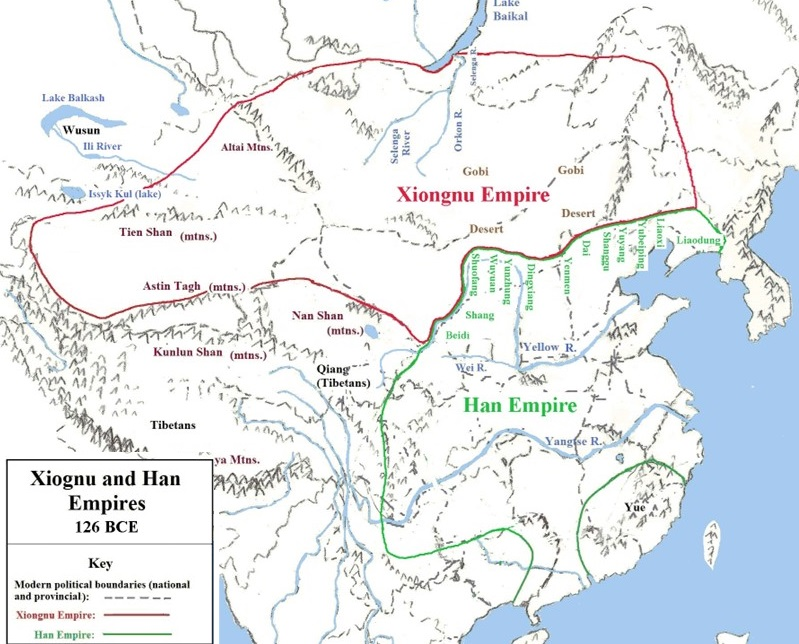
\includegraphics[width=0.8\textwidth]{ConfucianismeTaoismeBouddhismeChinois/Images/xiognu Han.jpg}

    \label{fig:enter-label}
\end{figure}


A la fin du IIIè siècle avant notre Ere, un véritable empire, du lac Baikal jusqu'à la Corée. Soit au début de l'Empire Han. Ils vont lutter l'un contre l'autre. Un vrai problème pour les empereurs Han.


%----------------------------------------------------------
\subsubsection{mission diplomatique avec les Yuezhi}
\begin{figure}[!h]
    \centering
    \sidecaption{Expansion Han. On voit le Kuchan à l'Ouest. On voit les Yuezhi à l'ouest. On voit le corridor de la route de la soie}
    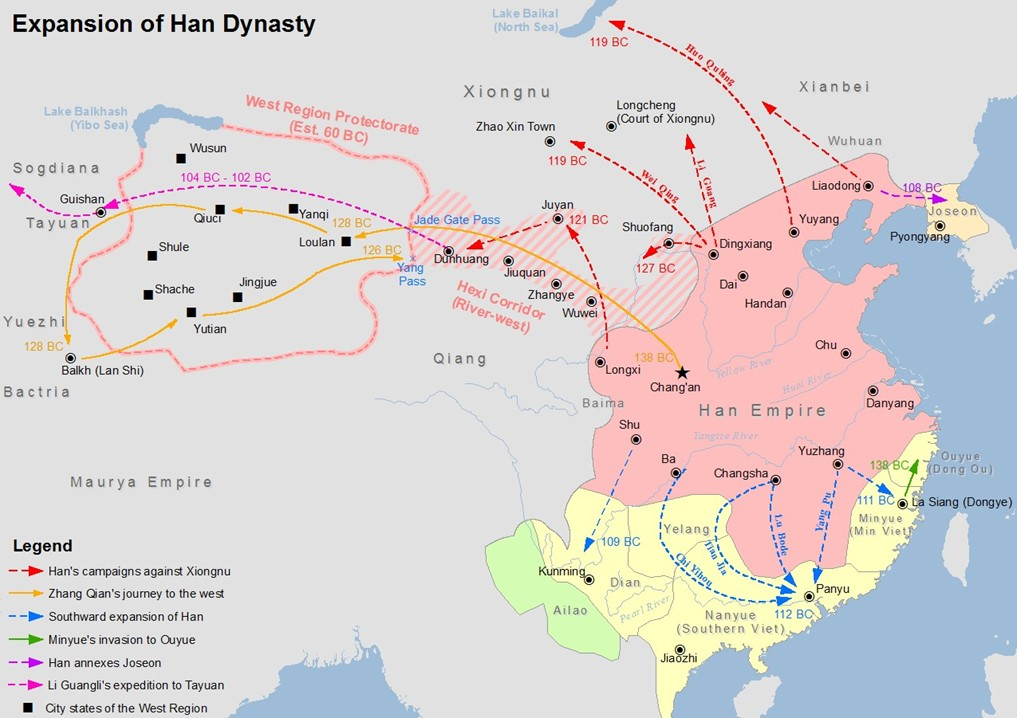
\includegraphics[width=0.8\textwidth]{ConfucianismeTaoismeBouddhismeChinois/Images/HanExpansion.jpg}

    \label{fig:enter-label}
\end{figure}

 

\begin{itemize}
   
   \item 	La politique offensive et expansionniste de l’empereur Wu (r. 141-87 av. J.-C.)
   \item 	La mission diplomatique de Zhang Qian (mort en 113 av. J.-C.) visant à négocier une alliance avec les Yuezhi contre les Xiongnu.
   \item Les \textbf{Yuezhi}: population de pasteurs, les Yuezhi nomadisaient, à l’avènement des Han, sur un vaste territoire correspondant au Xinjiang actuel. Chassés par les Xiongnu vers 170-160, ils nomadisèrent dès lors entre le lac Balkash et la vallée de l’Ili avant de descendre vers la vallée de l’Oxus au sud. Vers 130 avant notre ère, ils franchirent l’Oxus et occupèrent tout le territoire de la Bactriane grecque (sud de la Sogdiane, Bactriane et est de la Margiane). Ils y fondèrent au 1er siècle de notre ère l’Empire kuchan, étendant leur puissance sur toute l’Inde du Nord.
\end{itemize}

\paragraph{Une mission diplomatique de Zhang Qian vers les Yuezhi}

\begin{figure}[!h]
    \centering
        \sidecaption{Pays décrits dans les rapports de Zhang Qian (mort en 113 av. J.-C.).
Ceux que Zhang a lui-même visités sont soulignés en bleu. source wikipedia}
    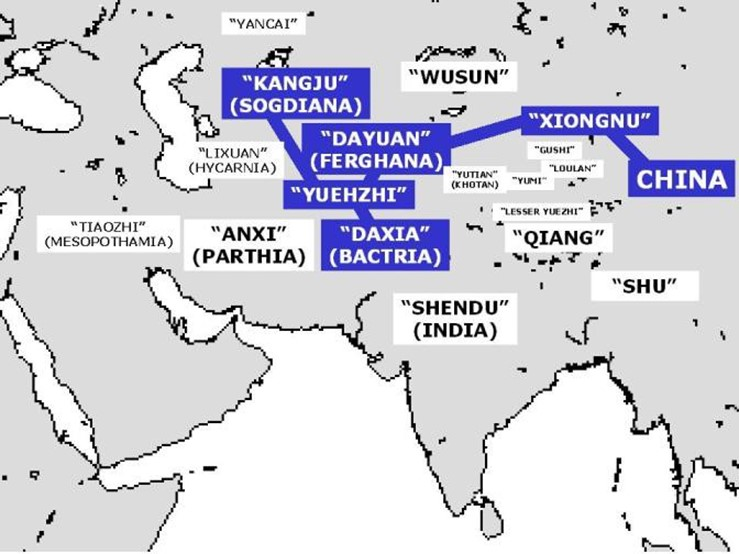
\includegraphics[width=0.8\textwidth]{ConfucianismeTaoismeBouddhismeChinois/Images/PaysZhan.jpg}

    \label{fig:enter-label}
\end{figure}

%----------------------------------------------------------
 \subsubsection{L’empire kuchan (1er – 3ème siècle de notre ère)}
\label{sec:Kuchan}
Cet empire a été créé par les Kouchans, qui ont eu des contacts diplomatiques avec Rome, l’Empire perse des Sassanides et la Chine et, pendant plusieurs siècles, furent au centre des échanges entre Orient et Occident. Il désignait soit l’une des cinq tribus des Yuezhi (月氏) soit l'une des cinq principautés soumises aux Yuezhi.

Seconde moitié de l'empire Han, coexistence avec les Han. 
\begin{figure}[!h]
    \centering
    \sidecaption{L'empire Kush}
    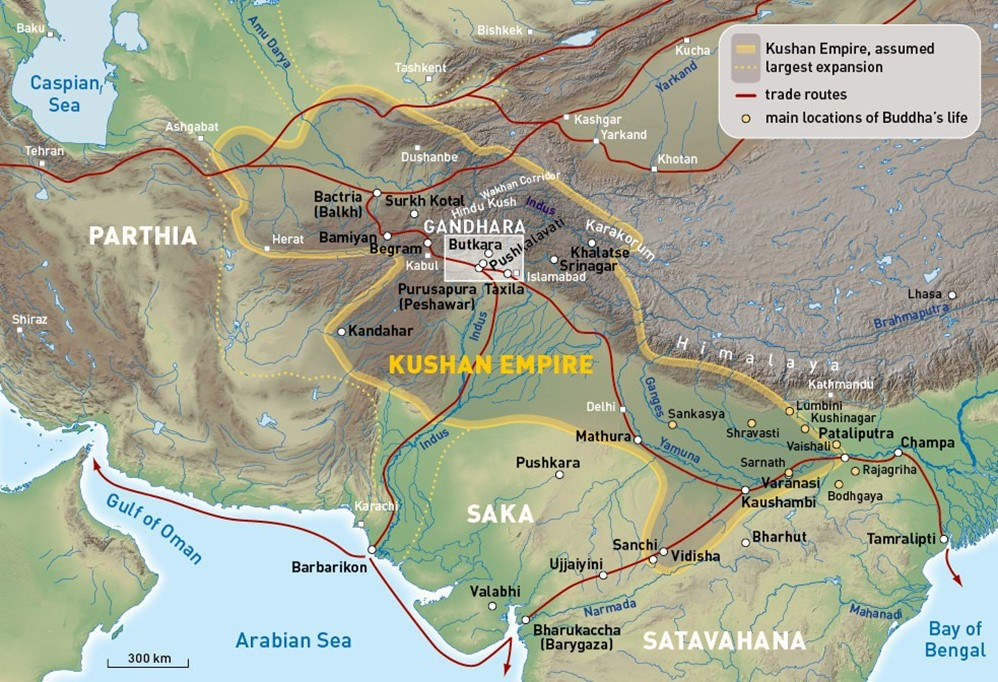
\includegraphics[width=0.8\textwidth]{ConfucianismeTaoismeBouddhismeChinois/Images/KushEmpire.jpg}

    \label{fig:enter-label}
\end{figure}

 \paragraph{role centrale de relier la Chine et l'empire Romain} 

 \paragraph{le Bouddhisme, religion Kushan} Dans les caravanes de marchands, probablement des moines Bouddhistes.




%----------------------------------------------------------
\subsection{L’assimilation du bouddhisme par la culture chinoise}

\paragraph{trois grandes étapes}

Les grandes étapes:
\begin{itemize}
    \item  	\textbf{Période de préparation} (des origines jusqu’au début du 4ème siècle)
Période marquée par une certaine ambiguïté des premières motivations chinoises fondées sur le désir d’immortalité et sur le goût des lettrés pour les discussions ésotériques; confusion entre le bouddhisme et le taoïsme. Le Bouddhisme serait une forme du Taoisme.

 \item 	\textbf{Période d’implantation} (4ème – 6ème siècles)
Le bouddhisme se diffuse largement dans une Chine divisée en deux parties: le Nord dominé par des régimes étrangers et le Sud où règnent des dynasties chinoises; appropriation du bouddhisme avec des nouvelles traductions de textes bouddhiques permettant de séparer le bouddhisme du taoïsme.
 


 \item 	\textbf{Période de sinisation ou d’assimilation véritable} (seconde moitié du 6ème siècle – fin du 10ème siècles), sous les \textit{dynasties Sui et Tang}.  Le bouddhisme pénètre toutes les couches de la société et se sinise entièrement. Les différents courants, ou « écoles », bouddhiques se forment au fil du temps.
 
\end{itemize}

\subsection{Période de préparation (des origines jusqu’au début du 4ème siècle)}

\mn{Kenneth CH’EN, Histoire du Bouddhisme en Chine, traduit de l’anglais par Dominique Kych, Paris : Les Belles Lettres, 2015, p. 58.}


\begin{figure}[!h]
    \centering
    \sidecaption{Le Bouddhisme sous les Han (I-IIè siècle). On connait très centres : Pencheng, Luoyang et Juaozhou dans le Tonkin. }
    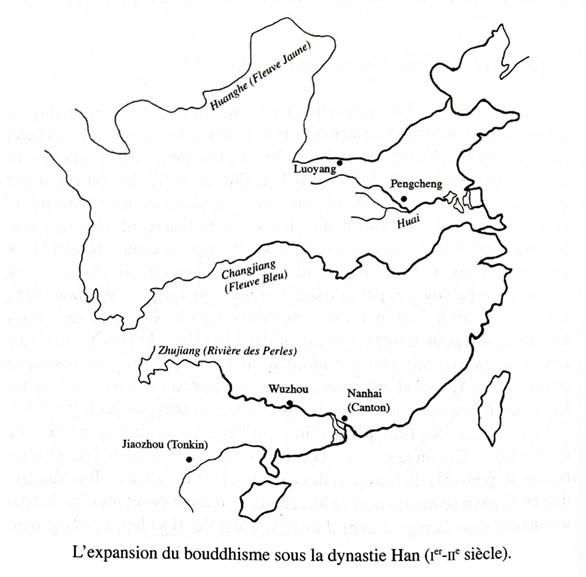
\includegraphics[width=0.8\textwidth]{ConfucianismeTaoismeBouddhismeChinois/Images/BouddhismeHan.jpg}

    \label{fig:enter-label}
\end{figure}

\paragraph{le centre le plus important est celui de Luoyang}
\paragraph{des Bouddhistes au palais} On met Laozi et Bouddha à côté. 
 


 \paragraph{Premiers moines étrangers arrivés en Chine }
investis dans la traduction de textes bouddhiques:
\begin{itemize}
    \item  	\textbf{An Shigao 安世高 }  : Premier grand traducteur de textes bouddhiques en chinois. D’origine parthe arsacide, An Shigao était, semble-t-il, un prince ayant renoncé au trône pour se faire religieux. Il arriva en 148 à Luoyang, alors capitale des Han postérieurs.
Ses traductions relevaient toutes du hīnayāna  dont beaucoup exposent des pratiques méditatives proches de celles du taoïsme.
\begin{Def}[hīnayāna]
    Petit véhicule, ancien. Appliqué à tous les courants qui semblaient privilégier, comme but de la pratique, la libération individuelle plutôt que la libération universelle de tous les êtres, et dont le seul survivant actuel est le theravāda. Ce terme peut parfois avoir une connotation péjorative, définissant le hīnayāna comme « égoïste » par rapport au mahāyāna « altruiste ». hīna : déficient mais on le traduit par petit pour plus de neutralité.
    La langue est le \textit{pali}
\end{Def}
Il a converti un chinois, premier moine bouddhiste chinois.
 \item 	\textbf{Zhilou jiachan}     ou Zhi Chan   : Kuchan arrivé à Luoyang vers 167. A la différence d’Anshigao, Zhi Chan s’intéresse d’abord aux textes de la prajñāparamitā (la perfection de sagesse ou connaissance transcendante), un ensemble de textes relevant du mahāyāna.
\begin{Def}[mahāyāna]
    Mot sanskrit signifiant grand moyen de progression ou \textit{Grand Véhicule} et désignant une forme du bouddhisme, qui prit naissance vers le début de notre ère. Le mahayana est plus métaphysique que le bouddhisme antérieur, dès lors dénommé hinayana, ou « Petit Véhicule». La langue est le \textit{sanskrit}
\end{Def}
\end{itemize}


\paragraph{les points de convergence avec le Taoisme}
\begin{itemize}
    \item rites se ressemblent
    \item les rites privés : méditation, contrôle du souffle, abstinence de certains aliments.
    \item le bouddhisme vise au renoncement au luxe, et le Taoisme également : rester à l'égard des diversions. 
\end{itemize}
Mais le risque, c'est de ne pas véritablement rentrer dans le bouddhisme.


 \subsection{Obstacles rencontrés dans l’assimilation de la doctrine bouddhique par la culture chinoise:}

 
 \paragraph{obstacle au niveau des langues }	
Méthode de traduction employée dans cette période: « geyi » 	格義  (appariement des notions). 
\mn{Hajime NAKAMURA, Ways of Thinking of Eastern Peoples: India-China-Tibet-Japan, trad. Philip Wiener, Honolulu: The University of Press of Hawaii, 1971.}

Deux exemples :
\begin{itemize}
    \item Non-agir est utilisé pour traduire \textit{Nirvana}
    \item parfait en sanskrit, devient \textit{onde} en chinois, état parfait
    
\end{itemize}
Le Chinois garde toujours la même forme, au pluriel, au cas, le temps. Alors que l'Inde, flexionnel.
 \paragraph{des modes de pensée}



 
 


\paragraph{choc de culture} Les moines bouddhistes quittent leur famille. Difficilement acceptable par les chinois.

\begin{Def}[chujia 出家]
     Quitter sa famille (pour entrer au monastère) : se faire bonze ou bonzesse; renoncer au monde; entrer en religion; entrer dans les ordres. 
\end{Def}
\begin{itemize}
    \item Analyse psychologique très poussée en sanskrit, alors que ce n'est pas un sujet pour les chinois. 
    \item Le simple fait que le bouddhisme soit d'origine \textit{barbare}, est un frein. 
    \item la notion économique, la mendicité est un concept difficile pour les chinois.
\end{itemize}

\paragraph{Au niveau des traditions}
Lihuo lun (Dialogues pour dissiper la confusion) de Mouzi (Maître Mou). 

 \subsubsection{deux courants}
A la fin de la dynastie Han, deux courants s’étaient déjà dégagés au sein du bouddhisme.
\begin{itemize}
    \item  	Le premier, représenté par l’école du \textbf{dhyāna}, mettait l’accent sur le contrôle de l’esprit, la concentration et la suppression des désirs. L’école se fondait principalement sur les textes traduits par An Shigao et était de nature hīnayāna.
    
    \item	À l’opposé, l’école de la \textbf{prajñā}, fondée en grande partie sur les textes traduis par Zhi Chan, était plutôt d’inspiration mahāyāna et se consacrait surtout à sonder, derrière le voile des apparences, la nature de Bouddha et la réalité ultime. C'est lui qui va devenir la forme principale du bouddhisme en Chine. 
\end{itemize}

 





\subsection{Période de division après la chute des Han (220-581)}
Après la chute des Hans, une période très longue, en 581. 

\subsubsection{d'abord trois royaumes}

\begin{figure}[!h]
    \centering
    \sidecaption{Période des Trois royaumes (220-265). 
Jin occidentaux (265-316) }
    \includegraphics[width=0.8\textwidth]{ConfucianismeTaoismeBouddhismeChinois/Images/TroisRoyaumes.png}
 
    \label{fig:enter-label}
\end{figure}
 il y a ensuite unification mais rapide de l'empire sous les Jin.

 
\subsubsection{Dynastie du Nord et du Sud}
Le Nord est envahi par des étrangers. Les dynasties chinoises restent au Sud. Une dynastie rétablit les Jin, les Jin orientaux. 

\begin{figure}[!h]
    \centering
    \sidecaption{
Période des Dynasties du Nord et du Sud (317-589)
Période d’implantation du bouddhisme en Chine (4ème – 6ème siècles) }
    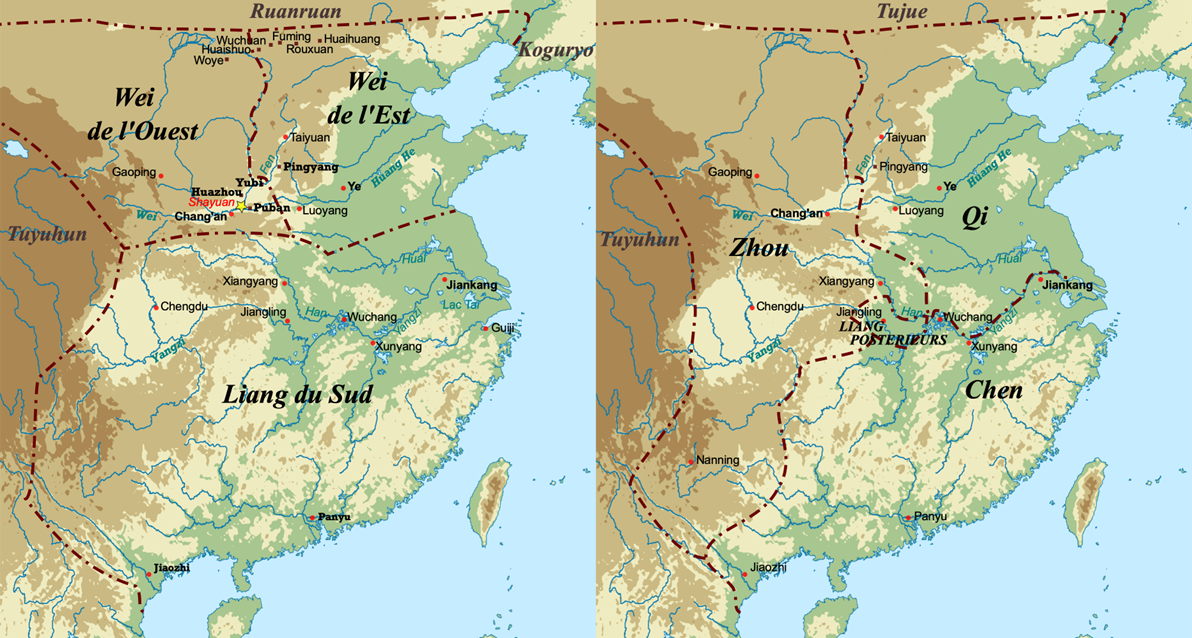
\includegraphics[width=0.8\textwidth]{ConfucianismeTaoismeBouddhismeChinois/Images/Dynastie3.png}
 
    \label{fig:enter-label}
\end{figure}

C'est dans cette période de Chaos que le Bouddhisme s'implante dans la société chinoise.

\subsection{dynastie du Nord et du Sud}
\begin{figure}[!h]
    \centering
    \sidecaption{
Période des Dynasties du Nord et du Sud (317-589)}
    \includegraphics[width=0.8\textwidth]{ConfucianismeTaoismeBouddhismeChinois/Images/DynastiesNord.png}
 
    \label{fig:enter-label}
\end{figure} 


\subsection{une différence de Bouddhisme}
\begin{figure}[!h]
    \centering
        \sidecaption{peinture de causeries où l'on voit les bouddhistes sans cheveux et les lettrés avec des chapeaux. Au début, très choquant pour les chinois de raser ses cheveux car la piété filiale requiert de respecter les cheveux, qui viennent des parents}
    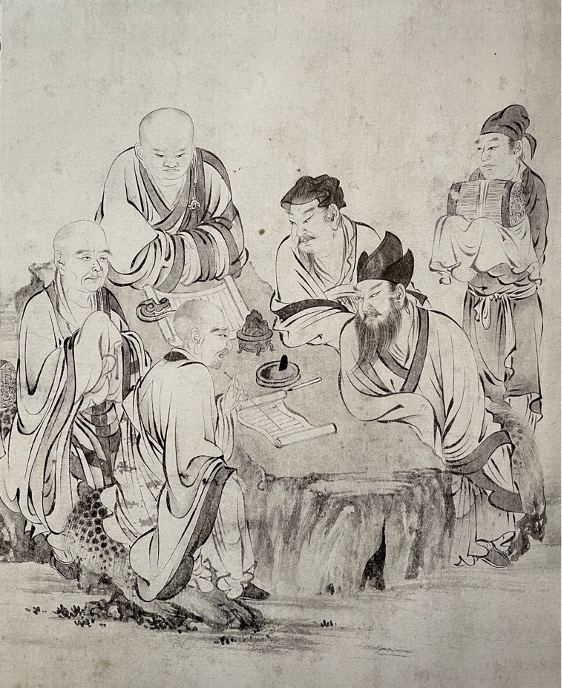
\includegraphics[width=.5\textwidth]{ConfucianismeTaoismeBouddhismeChinois/Images/causeriesud.jpg}

    \label{fig:enter-label}
\end{figure}

\paragraph{Dans le Sud:} plus intellectuel.

\begin{itemize}
    \item L’« étude du Mystère », aussi dénommée par le terme « néo- taoïsme »
    \item « la causerie pure »
 Il n'est plus possible pour les pauvres de prendre une charge officielle. ils trouvent une occupation dans les loisirs, bains,...
\end{itemize}



 Forme de spontanéité et de liberté : recherche de moins de contraintes sociales. 

\textit{}


 \paragraph{Dans le Nord:}




\paragraph{Kumārajīva} L’arrivée de Kumārajīva
 (344 ou 350 – 413) ouvre une nouvelle phase de la traduction des textes bouddhiques en langue chinoise. Il est indien, sa mère est une princesse. Il est connu pour ses prouesses intellectuelles. Les chinois le capturent pendant 17 ans. Il apprend le chinois. Finalement, il décide de rester en Chine et se déplace dans la ville de : 
 Il passe 12 ans de sa vie à traduire en Chinois, gros projet bien organisé avec toute équipe (certains théologies, certains comparent le texte avec les précédentes traductions, d'autres copient...). 
Parmi les textes qu’il a traduits:
\begin{itemize}
    \item  	Le \textit{Sutra du Lotus}; le \textit{Sutra de Vimalakīrti}, textes fondamentaux pour les études
 \item 	les \textit{trois traités fondamentaux de l’école Madhyamika} fondée par Nāgārjuna: le Traité en 100 versets, le Traité de la voie moyenne et le Traité des douze portes.
\end{itemize}


\mn{bcp de moines étrangers continuent à entrer en Chine pendant cette période et vont de-taoiser le vocabulaire}

\paragraph{liens entre nord et Sud} les traductions du nord se diffusent dans toute la Chine, malgré la période de trouble.


 \subsection{Période de sinisation ou d’assimilation véritable}

Période de sinisation ou d’assimilation véritable (seconde moitié du 6ème siècle – fin du 10ème siècles), sous les dynasties Sui ("sué") et Tang.

\paragraph{Commencent les examens pour les fonctionnaires} qui débutent sous les Sué. 
  



\begin{figure}[!h]
    \centering
    \sidecaption{
Dynastie des Sui (581- 618)}
    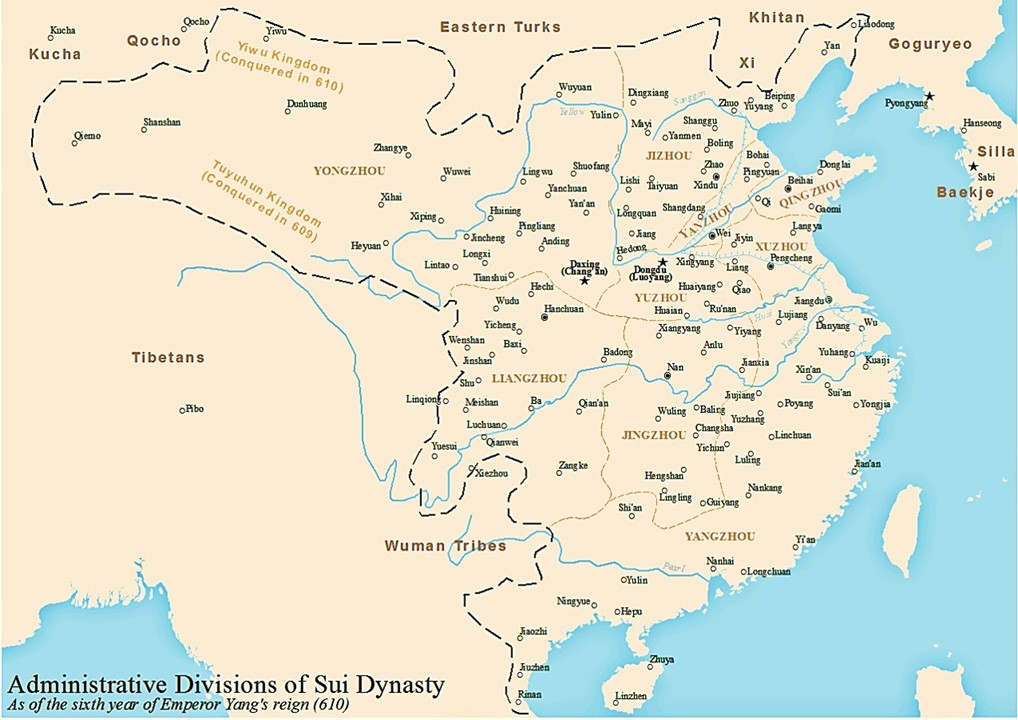
\includegraphics[width=0.8\textwidth]{ConfucianismeTaoismeBouddhismeChinois/Images/Sui.jpg}
 
    \label{fig:enter-label}
\end{figure} 



\begin{figure}[!h]
    \centering
    \sidecaption{Dynastie des Tang (618-907)}
    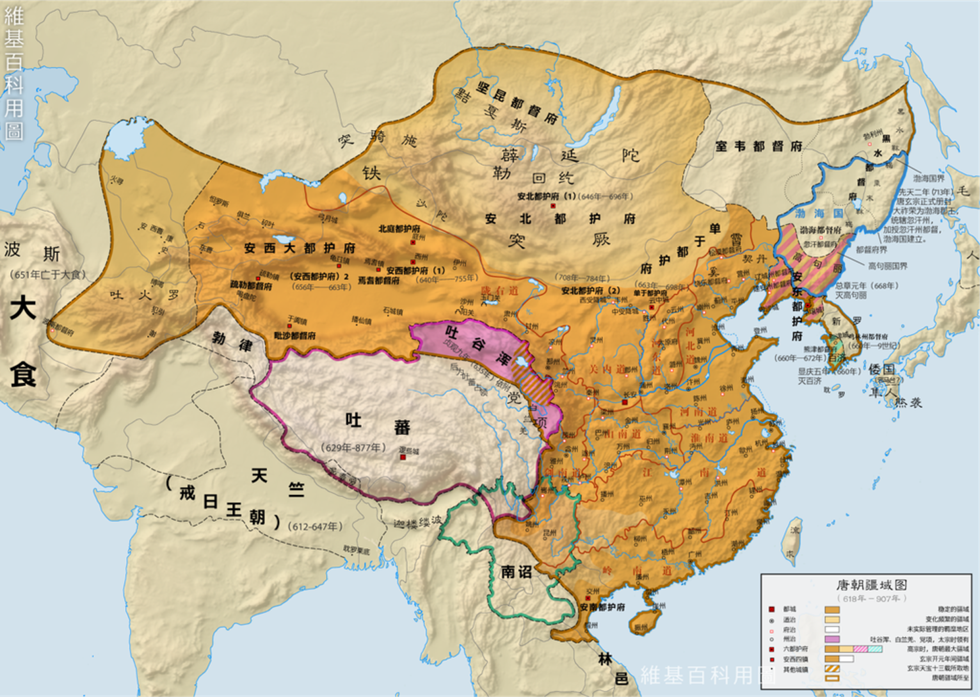
\includegraphics[width=0.8\textwidth]{ConfucianismeTaoismeBouddhismeChinois/Images/Tang.png}
 
    \label{fig:enter-label}
\end{figure} 




\section{Vocabulaire}

\begin{Def}[ ding 定]
    (Bouddh. – trad. du sanskr. samādhi « union, totalité, concentration totale de l’esprit » – transcr. phon. 三昧地 san mei di) 
    
    1. Concentration de l’esprit sur un objet unique par une diminution progressive de l’activité de l’esprit. 
    
    2.  État de conscience non dualiste, caractérisé par l’union, allant jusqu’à la non-différenciation entre le sujet et l’objet. 
\end{Def}
\begin{Def}[fa 法]
    Loi, légal ; droit ; (Philos. chin.) Loi ; légisme (法家 fajia) ; norme, règle ; modèle, exemplaire ; imiter ; méthodes, procédé. (Bouddh. – trad. du pâli dhamma et du sanskr. dharma « ordre; droit; usage; loi; doctrine religieuse » – trans. phon. chin. 達摩 da mo) 
    
    1. La loi cosmique, le « Grand Ordre » auquel notre monde est soumis et dont le principal aspect est la loi de la renaissance, associé au karma. 
    
    2. La doctrine du Bouddha qui, le premier, prit conscience de cette « Loi » et la formula 
    
    3. Le second des Trois Joyaux (triratna, 三寶 san bao) : le Bouddha, la Loi et la Communauté. 
    
    4. Manifestation de la réalité des choses ; phénomènes en général. 
    
    5. Pensées ; contenus psychiques ; idées ; reflets des phénomènes ds l’esprit humain. Ensemble des règles éthiques et des normes de comportement (vinaya–piṭaka).  
    
    6. Terme désignant les « facteurs existentiels », pierres angulaires de la personnalité empirique et de son univers, ds le hīnayāna ( 小乘 xiao sheng).
\end{Def}

\subsection{Xuanzang et les pélerins}

\paragraph{des le 3ème siècle} des pélerins font le voyage. Le premier chinois à l'avoir fait, c'est Faxian 

\begin{figure}[!h]
    \centering
    \sidecaption{Voyage de Faxian, Dominique LELIÈVRE, Voyageurs chinois à la découverte du monde– De l’Antiquité au XIXe siècle, Genève: Éditions OLIZANE, 2004, p. 58.c}    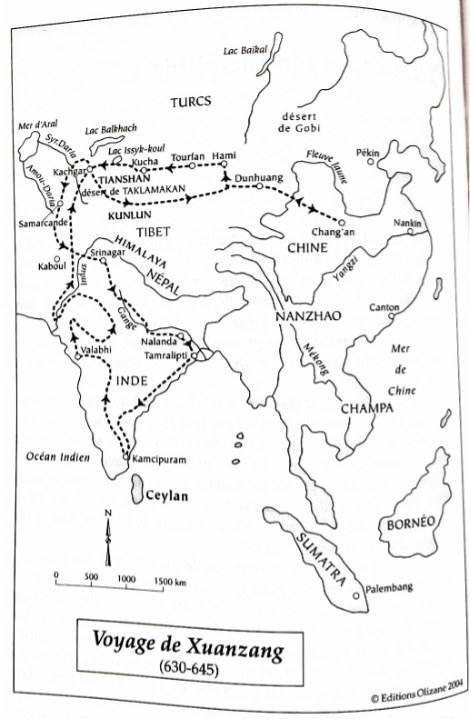
\includegraphics[width=.5\textwidth]{ConfucianismeTaoismeBouddhismeChinois/XuanzangVoyage2.jpg}

    \label{fig:enter-label}
\end{figure}
Pèlerins avant Xuanzang: à l’exemple de Faxian    (c. 338 -- c. 423 )	Foguo ji (Mémoire sur les royaumes bouddhiques)

\begin{Def}[Fo]
    Bouddhiste
\end{Def}
\paragraph{Xuanzang 玄奘 }
\begin{marginfigure}
    \centering
    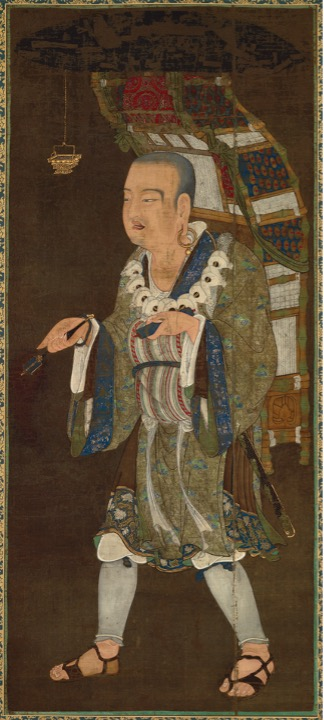
\includegraphics[width=\textwidth]{ConfucianismeTaoismeBouddhismeChinois/Xuanzang.jpg}
    \caption{Xuanzang}
    \label{fig:enter-label}
\end{marginfigure}

\paragraph{Voyage de Xuanzang}
 Il part en 630 à 28 ans. Il part clandestinement de Chine.
 

\begin{figure}[!h]
    \centering
        \sidecaption{Voyage de Xuanzang}
    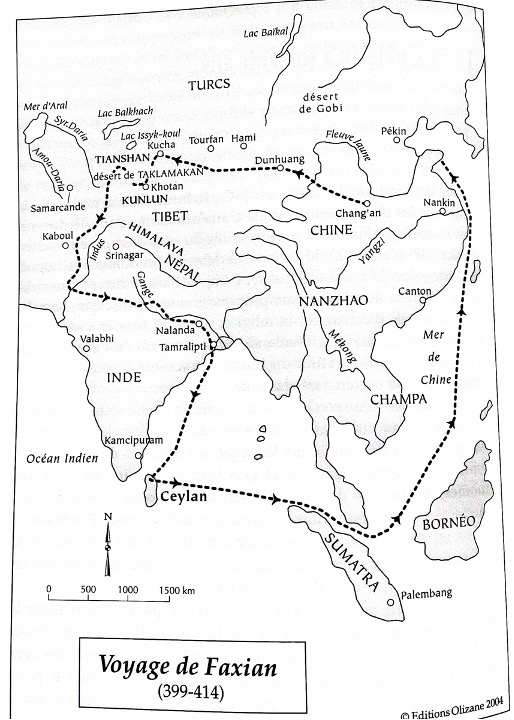
\includegraphics[width=.4\textwidth]{ConfucianismeTaoismeBouddhismeChinois/XuanzangInde.jpg}

    \label{fig:enter-label}
\end{figure}
•	Da Tang xiyu ji (Mémoire sur les Contrées occidentales à l’époque des grands Tang)

Il arrive à Nalanda, lieu saint du Grand Véhicule.
Il reste 5 ans à Nalanda. Il fait ensuite le tour des lieux saints de l'Inde. Il rencontre l'empereur Arsha(?).

Il rentre ensuite en Chine, est pardonné par l'empereur Taizong de son départ clandestin. 

\begin{Prop}[Pérégrination vers l'Ouest]
    Il est très connu du fait de \textit{la pérégrination vers l'Ouest } de Wu Cheng'en, avec un disciple de singe, de Cochon, de Singe. Dans ce roman, Xuanzang doit affronter les étapes grâce aux dieux taoïstes et bouddhistes. C'est un roman très profond car tout est métaphore des difficultés rencontrés lors de la pratique du bouddhisme.
\end{Prop}

\begin{Ex}[Métaphore de pérégrination vers l'Ouest]
    Difficulté à maitriser le souffle.
\end{Ex}

Au début et à la fin de chaque chapitre, il y a des poèmes qui explicitent les métaphores.

\subsection{les écoles bouddhistes à la fin des Tang}

Vers la fin des Tang, les différentes écoles bouddhiques qui s’affirment peuvent être rangées en trois groupes:
\begin{itemize}
    \item Le premier, enraciné dans le bouddhisme indien, compte quatre écoles : Chengshi (« Accomplissement de la vérité ») et Jushe (« Trésor métaphysique »), qui sont le prolongement des Sautrantika et des Sarvāstivādin dans le Petit Véhicule ; Sanlun (« Trois traités ») et Faxiang (« Caractères spécifiques des Dharma ») ou Weishi(« Rien que conscience »), qui représentent le Mādyamika et le Vijñānavāda du Grand Véhicule.
    \item Le deuxième regroupe les quatre écoles du bouddhisme chinois proprement dit :
    \item Tiantai (« Terrasse céleste »), Huayan (« La Guirlande de fleurs »), Chan (« Méditation ») et Jingtu (« Terre pure »).
    \item Le troisième groupe désigne deux écoles tardives Lüzong (école de la discipline) et Zhenyan (shingon en japonais), d’inspiration indienne.
\end{itemize}


\paragraph{Le Hīnayāna (Petit Véhicule) et le Mahāyāna (Grand Véhicule)}

\begin{Def}[véhicule ] - Yâna en sanskr.
    métaphore pour désigner le cheminement spirituel / exercices pour passer de l'ignorance à l'éveil.
\end{Def}




\begin{Def}[xiaosheng 小乘]
    (Bouddh. – ce terme traduit le sanskr. : \textit{hînayâna}) Petit véhicule, moyen inférieur de progression :	
    
    1. Nom donné par les partisans du 大乘 da sheng ou mahâyâna à la doctrine de tendance conservatrice du bouddhisme primitif. Ce terme est plus ou moins l’équivalent de Theravâda, « voie ou doctrine des Anciens ». 
    
    2. Bouddhisme dit du Sud, tel qu’il est pratiqué au Sri Lanka, en Birmanie, en Thaïlande et au Cambodge (mais le terme Hînayâna ayant un sens dépréciatif, ses adeptes préfèrent se désigner comme suivant le Theravâda).
\end{Def}

Toutes les écoles dans le monde appartiennent au Grand véhicule sauf dans le Sud de l'Inde. 

\begin{Def}[dasheng 大乘]
    (Bouddh.) Mahâyâna ou Grand Véhicule : considéré par ses adeptes comme un moyen plus efficace de salut que le Hînayâna (小乘 xiao sheng) ou Petit Véhicule. En Chine, au Tibet, en Mongolie, en Corée, au Japon, et ds presque tout le Viêtnam, le bouddhisme relève de la tradition du Mahâyâna.

    Une des variations du Grand véhicule, c'est le bouddhisme tibetain (nom : x? ).
\end{Def}

\paragraph{histoire du grand véhicule} dans le nord de l'Inde se développe une école de la sagesse. Le grand véhicule est influencé par cette école de la sagesse. Grands monastères dans le Nord de l'inde.
La littérature très abondante attachée au Grand Véhicule accorde la primauté aux textes de sagesse (prajñāparamitā sutra)

\begin{Def}[Prajñāparamitā]
    Prajñāparamitā (perfection de la sagesse transcendante)

    \begin{itemize}
        \item  	prajna : connaissance supérieure ou la meilleure, c’est-à-dire la connaissance directe de la vérité qui mène à la libération.
\item 	Paramita : actions transcendantes
    \end{itemize}

\end{Def}

On ne sait pas s'il y a eu un chisme entre les deux véhicules. Le grand véhicule peut être vu comme un développement du petit véhicule.
Ce grand véhicule apparaît à la même époque que l'introduction du bouddhisme en Chine. 

\paragraph{Madyamika - voie du milieu} 	Au 2ème siècle, Nāgārjuna commentera les prajñāparamitā sutra et fondera ainsi l’école philosophique du Madyamika (Voie du milieu).

 Au 4ème siècle, Asanga fondera une deuxième école philosophique mahayaniste, le Cittamatra (Rien que conscience), en s’appuyant sur d’autres sutra du Mahayana couchés par écrit aux 3ème et 4ème siècles.
 
 Le Madyamika et le Cittamatra constituent les deux courants principaux du Grand Véhicule.

\paragraph{les principales différences entre les véhicules}

\begin{itemize}
    \item  La perception du Bouddha
   \item L’idéal des bodhisattva par contraste avec les arhat
   \item 	La notion de la vacuité
\end{itemize}


bodhisattva : il s'agit d'être éveillé, des Bouddhas, qui décident de revenir sur terre pour aider leurs semblables à s'élever.

les arhats : dans le petit véhicule, ceux qui ont été au plus haut niveau. 

\paragraph{le Mahayana}

Dans le Mahayana, le Bouddha est transcendant : \textit{" acte phénoménal d'être supra-mondain. "} Il garde des aspects humains et divins. Doctrine des trois corps (Trikaya). 

\begin{Def}[sanshen 三身]
    (Bouddh. – traduction du sanskr. trikāya)	Les trois corps du Bouddha :	
    
    - fashen 法身 ou dharmakāya, le corps de la Loi, corps d’essence; ce corps constitue le corps essentiel unique de tous les bouddhas. 
    
    - bao shen 報身 ou sambhogakāya, le corps de rétribution; c’est le corps de félicité par lequel le Bouddha se manifeste aux bodhisattvas. 
    
    - hua shen 化身 ou nirmānakāya, le corps de métamorphose; c’est le corps apparent par lequel le Bouddha s’est manifesté dans l’histoire. 
    
    Cette doctrine des trois corps est une des doctrines fondamentales du mahāyāna ou Grand Véhicule (大乘 da sheng) 
\end{Def}


\paragraph{corps de la Loi} A la fois corps et enseignement. Selon le grand véhicule, cette nature de Bouddha est présent dans tous les êtres (pneuma ?). Nous sommes encore obscurcis. On peut donc être éveillé, on est déjà bouddha dans le grand véhicule et il faut en prendre conscience. Dans le petit véhicule, 

Corps de la Loi : Union ou unité de l'être avec la Loi cosmique.


\paragraph{corps de rétribution} Dans les représentations de Bouddhas, on voit le corps de retribution. 32 marques principales : boucles dans les "cheveux", bras touchent, langue très longue.


\begin{marginfigure}
    \centering
    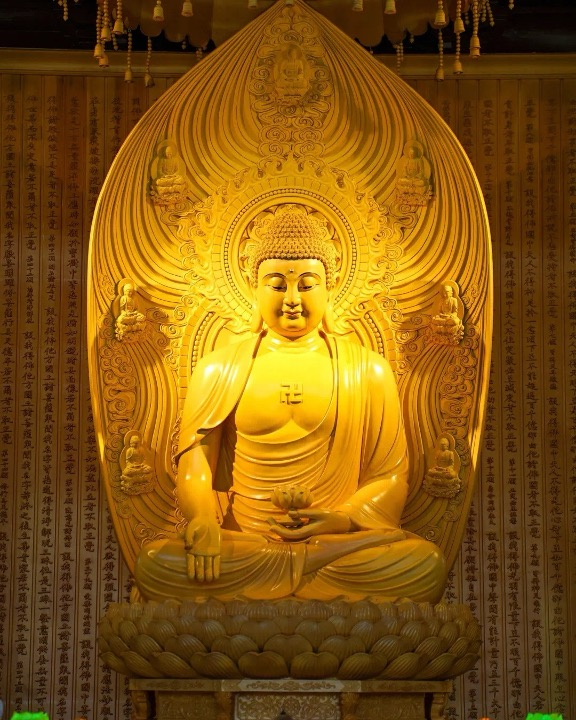
\includegraphics[width=\textwidth]{ConfucianismeTaoismeBouddhismeChinois/Images/bouddha.jpg}
    \caption{Corps de rétribution de Bouddha}
    \label{fig:enter-label}
\end{marginfigure}

\paragraph{le corps de métamorphose} il a pour base le corps de la loi, cosmos. Le Bouddha peut alors de manifester en fonction des besoins de chacun. 

\paragraph{Les bouddhas les plus populaires en Chine}




Amitābha (Amituofo) et sa Terre pure
Le bouddha Amitabha et sa Terre pure sont présentés principalement dans les Sukhāvatīvyūhasūtra (Sūtra des ornements de la terre bienheureuse)

•	Le grand Sukhāvatīvyūhasūtra ou Amitābhavyūhanāma Mahāyānasūtra (Wuliangshou jing)
•	Le petit Sukhāvatīvyūhasūtra dit « Sutra d’Amitabha »
